%!TEX TS-program = lualatex
%!TEX encoding = UTF-8 Unicode

%\frame[plain]{ % When including a large figure or table, you don't want to have the bottom and the top of the slides.
%\frame[shrink]{ % If you want to include lots of text on a slide, use the shrink option.

\begin{frame}
    \frametitle{FUSE (File System in User Space)}
    \begin{center}
        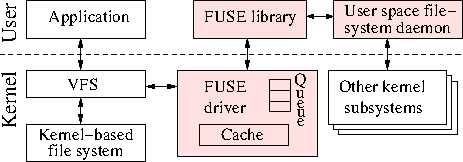
\includegraphics[width=.7\textwidth]{frames/img/fuse_arch}
    \end{center}
    
    \begin{itemize}
        \item simplifies writing file system drivers by avoiding kernel-level code
        \item mounting / unmounting can be done as a unprivileged user
        \item file ownership can be adjusted to enable unprivileged access to the filesystem
    \end{itemize}
    
    \note{
        \begin{itemize}
            \item library and suite of utilities for offline FS access
            \item runs a stripped down Linux appliance using libvirt and/or QEMU for FS-access
            \item mature ecosystem, many useful utilities
            \item used for Simics-externfs
        \end{itemize}
    }
\end{frame}